\documentclass[a4paper]{article}

\usepackage{fullpage} % Package to use full page
\usepackage{parskip} % Package to tweak paragraph skipping
\usepackage{amsmath}
\usepackage{hyperref}
\usepackage{amsmath,amsfonts,amsthm} % Math packages
\usepackage{graphicx}
\usepackage{listings}
\usepackage{color}
\usepackage{float}
\definecolor{codegreen}{rgb}{0,0.6,0}
\definecolor{codegray}{rgb}{0.5,0.5,0.5}
\definecolor{codepurple}{rgb}{0.58,0,0.82}
\definecolor{backcolour}{rgb}{0.95,0.95,0.92}
\definecolor{brown}{rgb}{0.59, 0.29, 0.0}
\definecolor{beaublue}{rgb}{0.74, 0.83, 0.9}
\definecolor{orange}{rgb}{1.0, 0.5, 0.0}
\definecolor{darkslategray}{rgb}{0.18, 0.31, 0.31}

\lstdefinestyle{mystyle}{
	backgroundcolor=\color{white},   
	commentstyle=\color{codegreen},
	keywordstyle=\color{blue},
	identifierstyle=\color{brown},
	numberstyle=\tiny\color{codegray},
	stringstyle=\color{orange},
	basicstyle=\footnotesize,
	breakatwhitespace=false,         
	breaklines=true,                 
	captionpos=b,                    
	keepspaces=true,                 
	numbers=left,                    
	numbersep=5pt,                  
	showspaces=false,                
	showstringspaces=false,
	showtabs=false,                  
	tabsize=2
}
\lstset{style=mystyle}

\title{AMATH 522: Problem Set 1}
\author{Jithin D. George}
\date{24/10/16}

\begin{document}

\maketitle

\section{Leslie Matrices and Euler-Lotkerra Formula}
 \begin{itemize}
 	\item  
 	\begin{lstlisting}[language=Matlab,frame=single]
	%% Problem Set 1 - Euler Lotkerra
	L = [ 0 1 5 0.5; 0.5 0 0 0; 0 0.9 0 0;0 0 0.95 0 ];
	N(:,1)= [100; 100; 100; 100;];
	for i=1:50
		N(:,i+1)=L*N(:,i);
	end;
	k=sum(N);
	t=1:51;
	figure;
	plot(t,log(k));
	title('Log of the total population size against time');
	xlabel('Time') % x-axis label
	ylabel('Log of the total population size') % y-axis label
	
	lamdase= polyfit(t,log(k),1);
	loglamda= lamdase(1,1);
	
	N0= N(1,:)./k;
	N1= N(2,:)./k;
	N2= N(3,:)./k;
	N3= N(4,:)./k;
	figure;
	plot(t,N0,t,N1,t,N2,t,N3);
	xlabel('Time') % x-axis label
	ylabel('Fractional population size of different ages') % y-axis label
	legend('Age 0', 'Age 1', 'Age 2', 'Age 3');
	legend('show')

 	\end{lstlisting}
 	
 	 \begin{figure}[h]
 	 	\centering
 	 	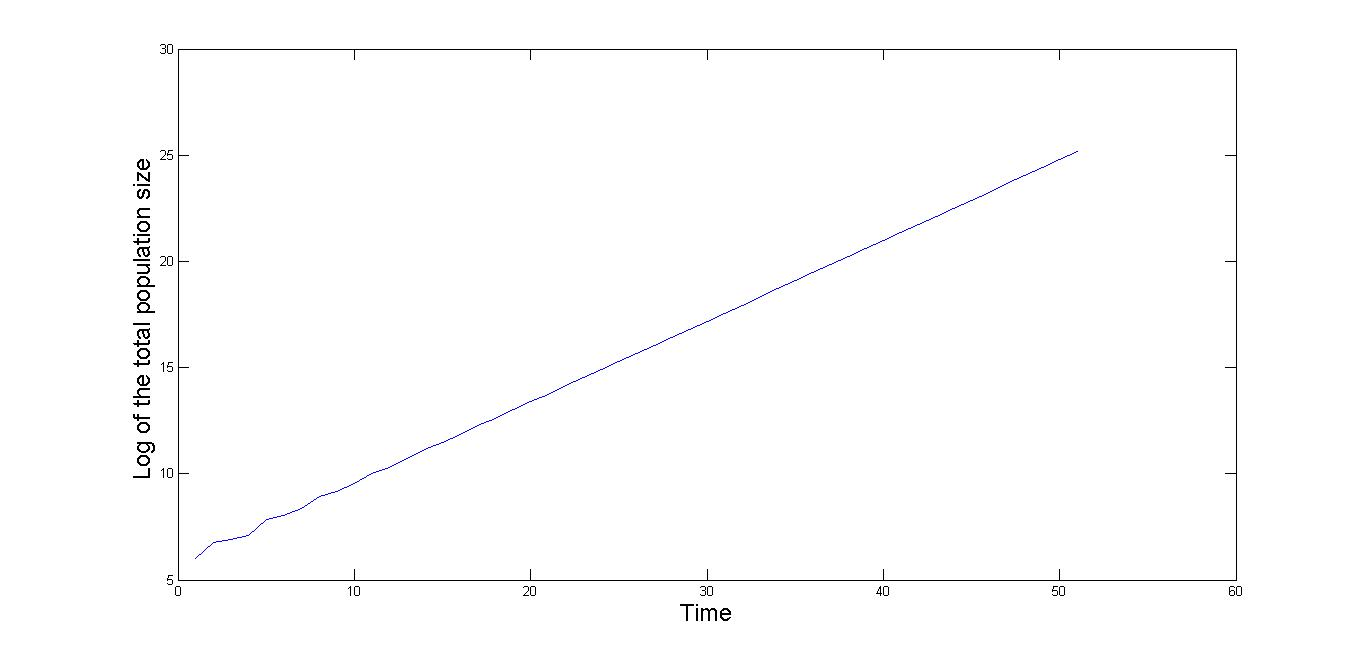
\includegraphics[width=12cm]{F1}
 	 \end{figure}
 
    $\lambda$ is obtained from polyfit as 1.4624.
 	
  	 \begin{figure}[h]
  	 	\centering
  	 	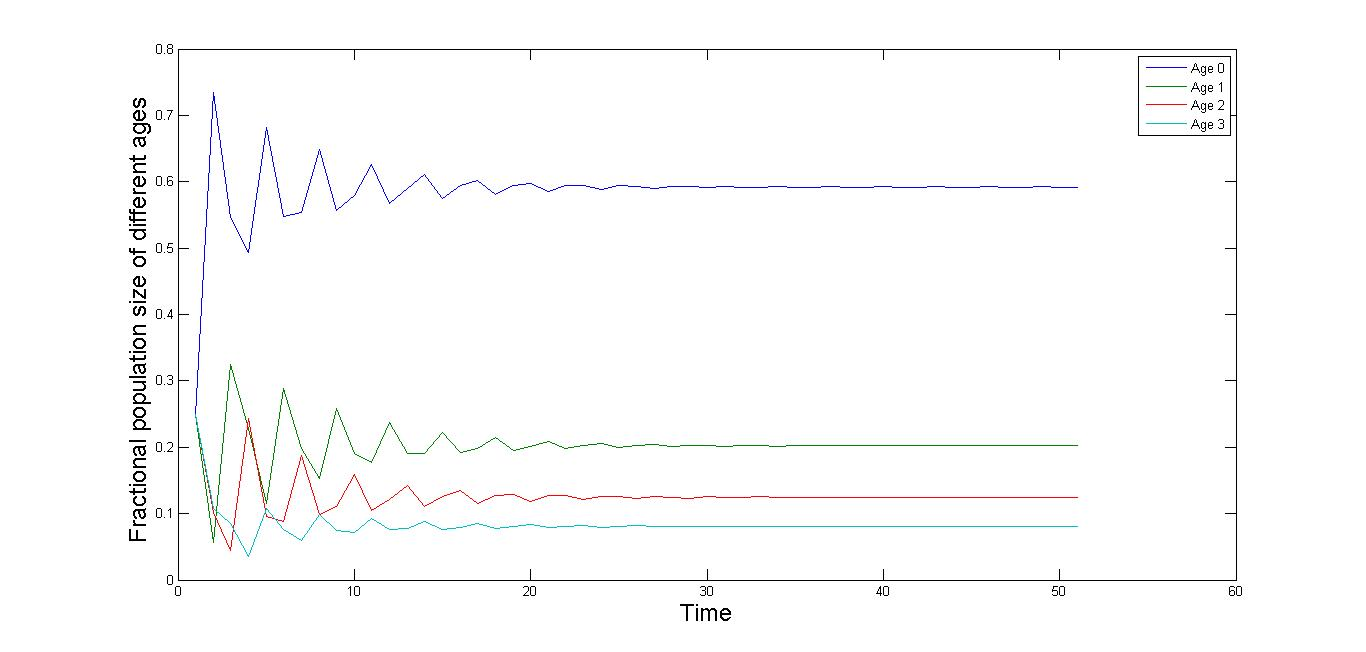
\includegraphics[width=12cm]{F2}
  	 \end{figure}
  	 	
 	\item   	
 	\[ f_0\lambda^3 +f_1 I_1 \lambda^2 +f_2 I_2 \lambda +f_3 I_3= 1\]
 	\begin{lstlisting}[language=Matlab,frame=single]
 
 	F = [ 0 1 5 0.5];
 	I = [1 0.5  0.45 0.45*0.95];
 	guess_min=0.0001; guess_max=10;
 	lambdabar = fzero(@(lambda) eulot(lambda,I,F),[guess_min,guess_max]);
 	
 	function f=eulot(lambda,Ia,fa);
	 	age=0:(length(Ia)-1);
	 	y=lambda.^(-(age+1));
	 	f=sum(y.*Ia.*fa)-1;
 	return;
 	\end{lstlisting}
 	
 	The $\lambda$ obtained is 1.4624
 \end{itemize}



\section{The Northern Spotted Owl}

\begin{itemize}
	\item The fecundities for ages 0 to 2 are zero. Hence,
	\[ \sum_{n=0}^{2}  I_a f_a =0     \] 
	and their survival probabilities don't matter in the Euler Lotkerra formula as long as their product is 0.0722
	\item 
	 	\begin{lstlisting}[language=Matlab,frame=single]
			%% Problem Set 1 - Owls
			clc; clear all;
			Lo = zeros(49);
			v=0.942.*ones(1,48);
			Lo=diag(v,-1);
			Lo(1,2:49)=0.24;
			Lo(2,1)=0.0722;
			No(:,1)= 100*ones(49,1);
			for i=1:49
				No(:,i+1)=Lo*No(:,i);
			end;
			k=sum(No);
			t=1:50;
			figure;
			plot(t,log(k));
			lam = polyfit(t,log(k),1);
			lamda =exp(lam(1,1));
			
			%Elasticity Matrix
			[Ri,BS]  = eigs(Lo);
			[Li,BS]  = eigs(transpose(Lo));
			Li=Li(:,1);%dominant left eigenvector
			Ri=Ri(:,1);%dominant right eigenvector
			es = sum(Li.*Ri);
			Elas =zeros(49);
			for i=1:49
				for j=1:49
					Elas(i,j) = (Lo(i,j)/BS(1,1))*(Li(i,1)*Ri(j,1)/es);
				end;
			end;
	 	\end{lstlisting}
	 	
	 	
	 	\item 
	 	The $\lambda$ obtained is 0.9398
	 	\item The elasticity for the fecundity values are close and small but not similar. They increase slightly as the age increases. This might be because the older generations may have more impact on breeding than the younger ones.
	 	
	 	The elasticity for survival probabilities is not the same either and decreases with age. A possible reason is that the older generations only contribute to the few generations after them while the younger generations can have larger impact. So, while managing them, the younger generations should have more attention since they have a larger control of the eigenvalues.
\end{itemize}

\section{Killer Whales}
\begin{itemize}
	\item
	 	\begin{lstlisting}[language=Matlab,frame=single]
		%% Problem Set 1 - Killer Whales
		clc; clear all;
		A=[ 0 0.0043 0.1132 0; 0.9775 0.9111 0 0 ; 0 0.0736 0.9534 0; 0 0 0.0452 0.9804];
		[L,B] =eigs(A);
		L =L(:,1);
		B=B(1,1);
		s = sum(L);
		x = 250/s;
		
		% Adults
		N=zeros(4,1000);
		N(:,1)=x.*L;
		hold on;
		t =1:1000;
		hi=0;
		for ha= 1:0.001:10
			hi=hi+1;
			for i=1:999
				N(:,i+1)=A*N(:,i);
				Int=N(3,i+1)-ha;
				if Int<0
					N(3,i+1) =0;
				else
				N(3,i+1)=Int;
				end;
				sub = sum(N(:,i+1));
				if sub<1
					disp(i);
					break;
				end
			end
			sk=sum(N(:,1:i));
			if sub<1
			 break;
			end ;
		end
		plot(1:i,sk); 
		xlabel('Time','FontSize',18) % x-axis label
		ylabel('Adult population with extinction harvesting','FontSize',18) % y-axis label
		
		%Juveniles
		N=zeros(4,1000);
		N(:,1)=x.*L;
		figure;
		hold on;
		t =1:1000;
		hi=0;
		for hj= 1:1:10
			hi=hi+1;    
			for i=1:999
				N(:,i+1)=A*N(:,i);
				Int=N(2,i+1)-hj;
				if Int<0
					N(2,i+1) =0;
				else
				N(2,i+1)=Int;
				end;
				sub = sum(N(:,i+1));
				if sub<1
					disp(i);
					break;
				end
			end
			sj=sum(N(:,1:i));
			if sub<1
				break;
			end ;
		end
		
		plot(1:i,sj); 
		xlabel('Time','FontSize',18) % x-axis label
		ylabel('Juvenile population with extinction harvesting','FontSize',18) % y-axis label
 	\end{lstlisting}
 	
  \item	 \begin{figure}[h]
  	 	\centering
  	 	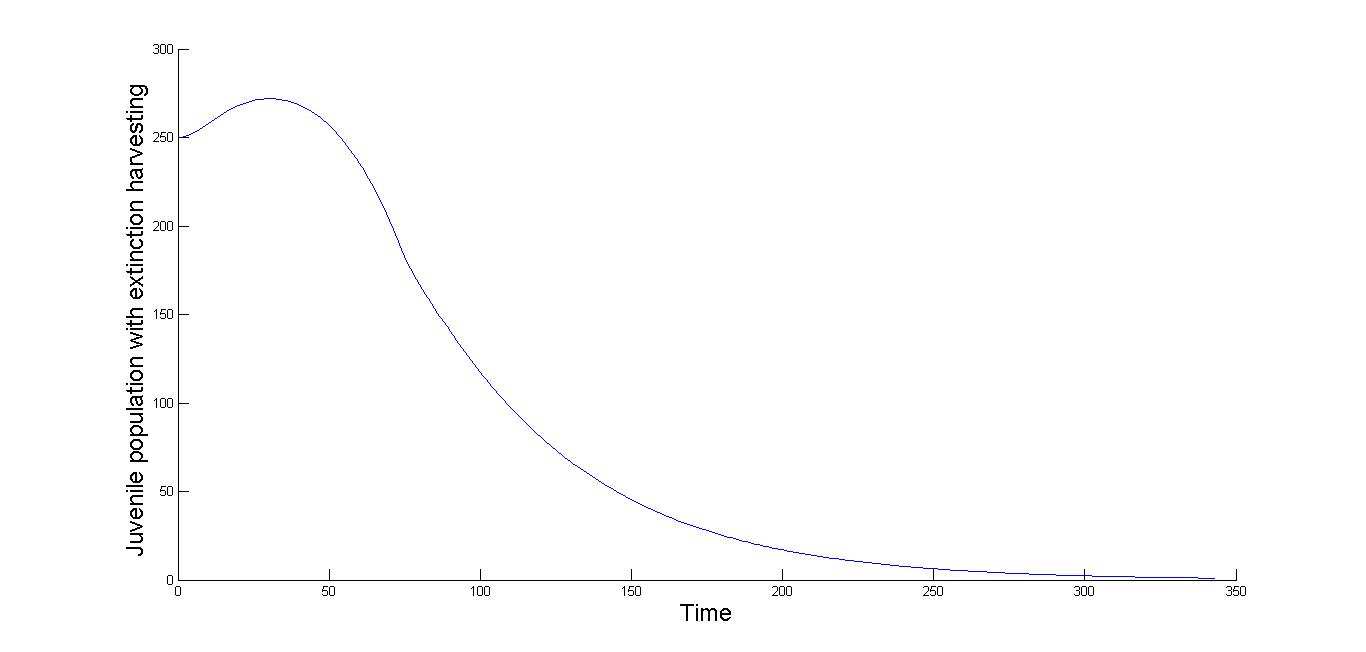
\includegraphics[width=12cm]{J}
  	 \end{figure}
  	 
  	 The maximum juvenile harvest is 5.310. Beyond this, the population goes extinct like the plot above.

  \item	 \begin{figure}[H]
  	 	\centering
  	 	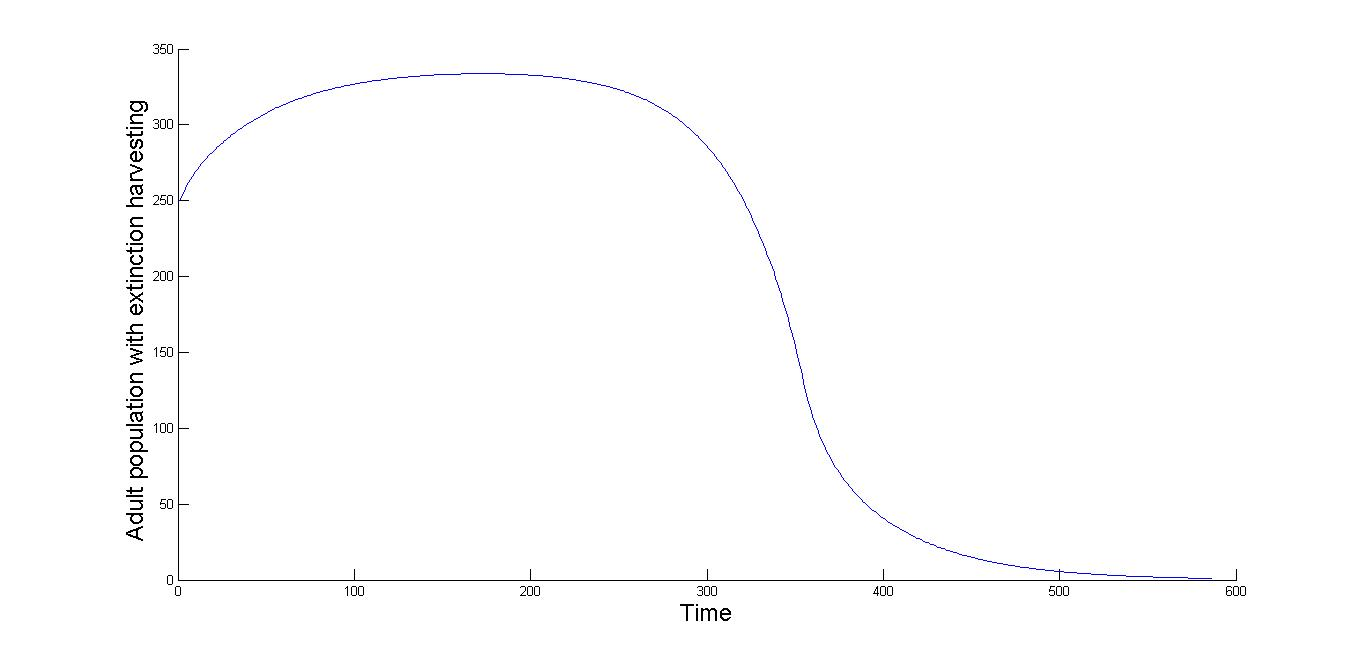
\includegraphics[width=12cm]{A}
  	 \end{figure}  	 
  	 The maximum adult harvest is 3.545. Beyond this, the population goes extinct like the plot above.
  	 \end{itemize}
\section{MATLAB Programming}

\begin{itemize}
	\item awgn()
	Adds white Gaussian noise to a vector signal or a matrix after specifying signal to noise ratio. Excellent for testing accuracy of algorithms in the midst of noise.
	\item contourf()
	A great way to plot a function that varies over a 2-dimensional domain.
\end{itemize}

\section{Project Warmup}

\begin{itemize}
	\item Panetta, J. C. "A logistic model of periodic chemotherapy." Applied mathematics letters 8.4 (1995): 83-86.
	\item This model serves to describe the effects of chemotherapeutic drugs on cancer cell growth and to find the necessary conditions for zero equilibrium (so as to destroy the cancer cells) and other equilibria for appropriate acceptable bone marrow deterioration. It uses a logistic differential equation to model the periodic chemotherapy.
	\item The model revolves around the following logistic differential equation.
	\[      \frac{dy(t)}{dt}= ry(t)\Big([1-b(t)] -\frac{y(t)}{K} \Big)  \]
	where 
	\begin{itemize}
		\item y(t) is the cell mass at time t.
		\item r is the cell growth rate.
		\item K is the carrying capacity.
		\item b(t) is a periodic function representing the chemotherapeutic effects.
	\end{itemize}
	\item One of the most important assumptions here is that the chemotherapeutic effects of the drug can be modeled by a continuous or piecewise continuous periodic function.
\end{itemize}


\end{document}